%=====Tips when editing and compiling this file:=====
%-Each time of edition, change the typesetting engine (the second blank in the heading section) to "XeLaTeX", to allow xeCJK package
%========Other tips=====
%-if console says there is error like:
%...
%l.64 ]{NotoSansSC}
%maybe this is due to lack of a comma in the previous []

%-May need to press Return (or Enter for PC) to apply the CV_CN.cls, etc., when console is compliling this tex file

%-learn about font sizes, styles /typefaceshere:
%https://www.overleaf.com/learn/latex/Font_sizes,_families,_and_styles
%https://www.overleaf.com/learn/latex/Font_typefaces

%-use CJK for chinese in section 'xeCJK with XeLaTeX' here:
%https://www.overleaf.com/learn/latex/chinese

%-supported CJK chinese fonts and other language fonts here: (or access this by the link at the end of the last linked page)
%https://www.overleaf.com/learn/latex/Questions/Which%20OTF%20or%20TTF%20fonts%20are%20supported%20via%20fontspec%3F#Chinese

%-中文简历撰写要点,见:
%https://zhuanlan.zhihu.com/p/154293833

%-make spaces:
%https://it.overleaf.com/learn/latex/Line_breaks_and_blank_spaces

%-find more free fonts here:
%https://fonts.google.com

%-load custom new fonts to xelatex, see guide:
%https://www.overleaf.com/learn/latex/Questions/I_have_a_custom_font_I'd_like_to_load_to_my_document._How_can_I_do_this%3F
%============================================

%Can be improved but not needed right now:
%-reduce space before each subsection header -> more compact, reduce number of pages, at best to 2 pages

%-to well-define package{cvcnfont} %use my custom fonts, defined in .sty file %I failed to load custom fonts/let definitions in .sty file apply to this .tex file; so I put fonts setting in .cls file temporarily

%-subsection headers enlarged wrt date or make dates smaller 

\documentclass[12pt]{CV_CN} %use my custom class, defined in .cls file


\usepackage{geometry}                % See geometry.pdf to learn the layout options. There are lots.
\geometry{letterpaper}                   % ... or a4paper or a5paper or ... 
%\geometry{landscape}                % Activate for for rotated page geometry
%\usepackage[parfill]{parskip}    % Activate to begin paragraphs with an empty line rather than an indent
\usepackage{graphicx}
\usepackage{amssymb}

\usepackage{wrapfig}

\usepackage{enumitem} %allow adjusting \topsep, \itemsep, \partopsep, \parsep for itemization
%see guides here:
%https://tex.stackexchange.com/questions/300340/topsep-itemsep-partopsep-parsep-what-do-they-each-mean-and-what-about
%and others about item spacing:
%https://tex.stackexchange.com/questions/10684/vertical-space-in-lists


% Will Robertson's fontspec.sty can be used to simplify font choices.
% To experiment, open /Applications/Font Book to examine the fonts provided on Mac OS X,
% and change "Hoefler Text" to any of these choices.

%\usepackage{fontspec,xltxtra,xunicode}
%\defaultfontfeatures{Mapping=tex-text}
%\setromanfont[Mapping=tex-text]{TrajanPro-Regular.otf} %replace Hoefler Text
%\setsansfont[Scale=MatchLowercase,Mapping=tex-text]{Gill Sans}
%\setmonofont[Scale=MatchLowercase]{Andale Mono}

%\usepackage{xeCJK} %allow Chinese, Japanese and Korean
%\setCJKmainfont[BoldFont=FandolSong-Bold.otf]{AdobeSongStd-Light.otf} %or use FandolSong-Regular.otf
%\setCJKsansfont[BoldFont=FandolHei-Bold.otf]{FandolHei-Regular.otf}
%\setCJKmonofont{FandolFang-Regular.otf}
%\newCJKfontfamily\kaiti{FandolKai-Regular.otf}
%this font-setting codes are from:
%https://tex.stackexchange.com/questions/223893/how-do-i-find-out-what-chinese-fonts-are-installed-with-my-mactex-installation
%and from this template:
%https://www.overleaf.com/latex/templates/chinese-resume-template-zhong-wen-jian-li-mo-ban/fbdypsjmgwbb

\usepackage{hyperref}
\hypersetup{
    colorlinks=True,
    linkcolor=black,
    filecolor=black,      
    urlcolor=black
}
%turn all hyperlinks to black to make page look neat

\documentclass{CV_CN}

\begin{document}
\name{傅时敏}{FU, Shimin}
\begin{wrapfigure}{t}{0.35\textwidth} %this figure will be at the top; {2nd argumant} =width of figure, but can be covered by width specified when including the image as below
    \centering
    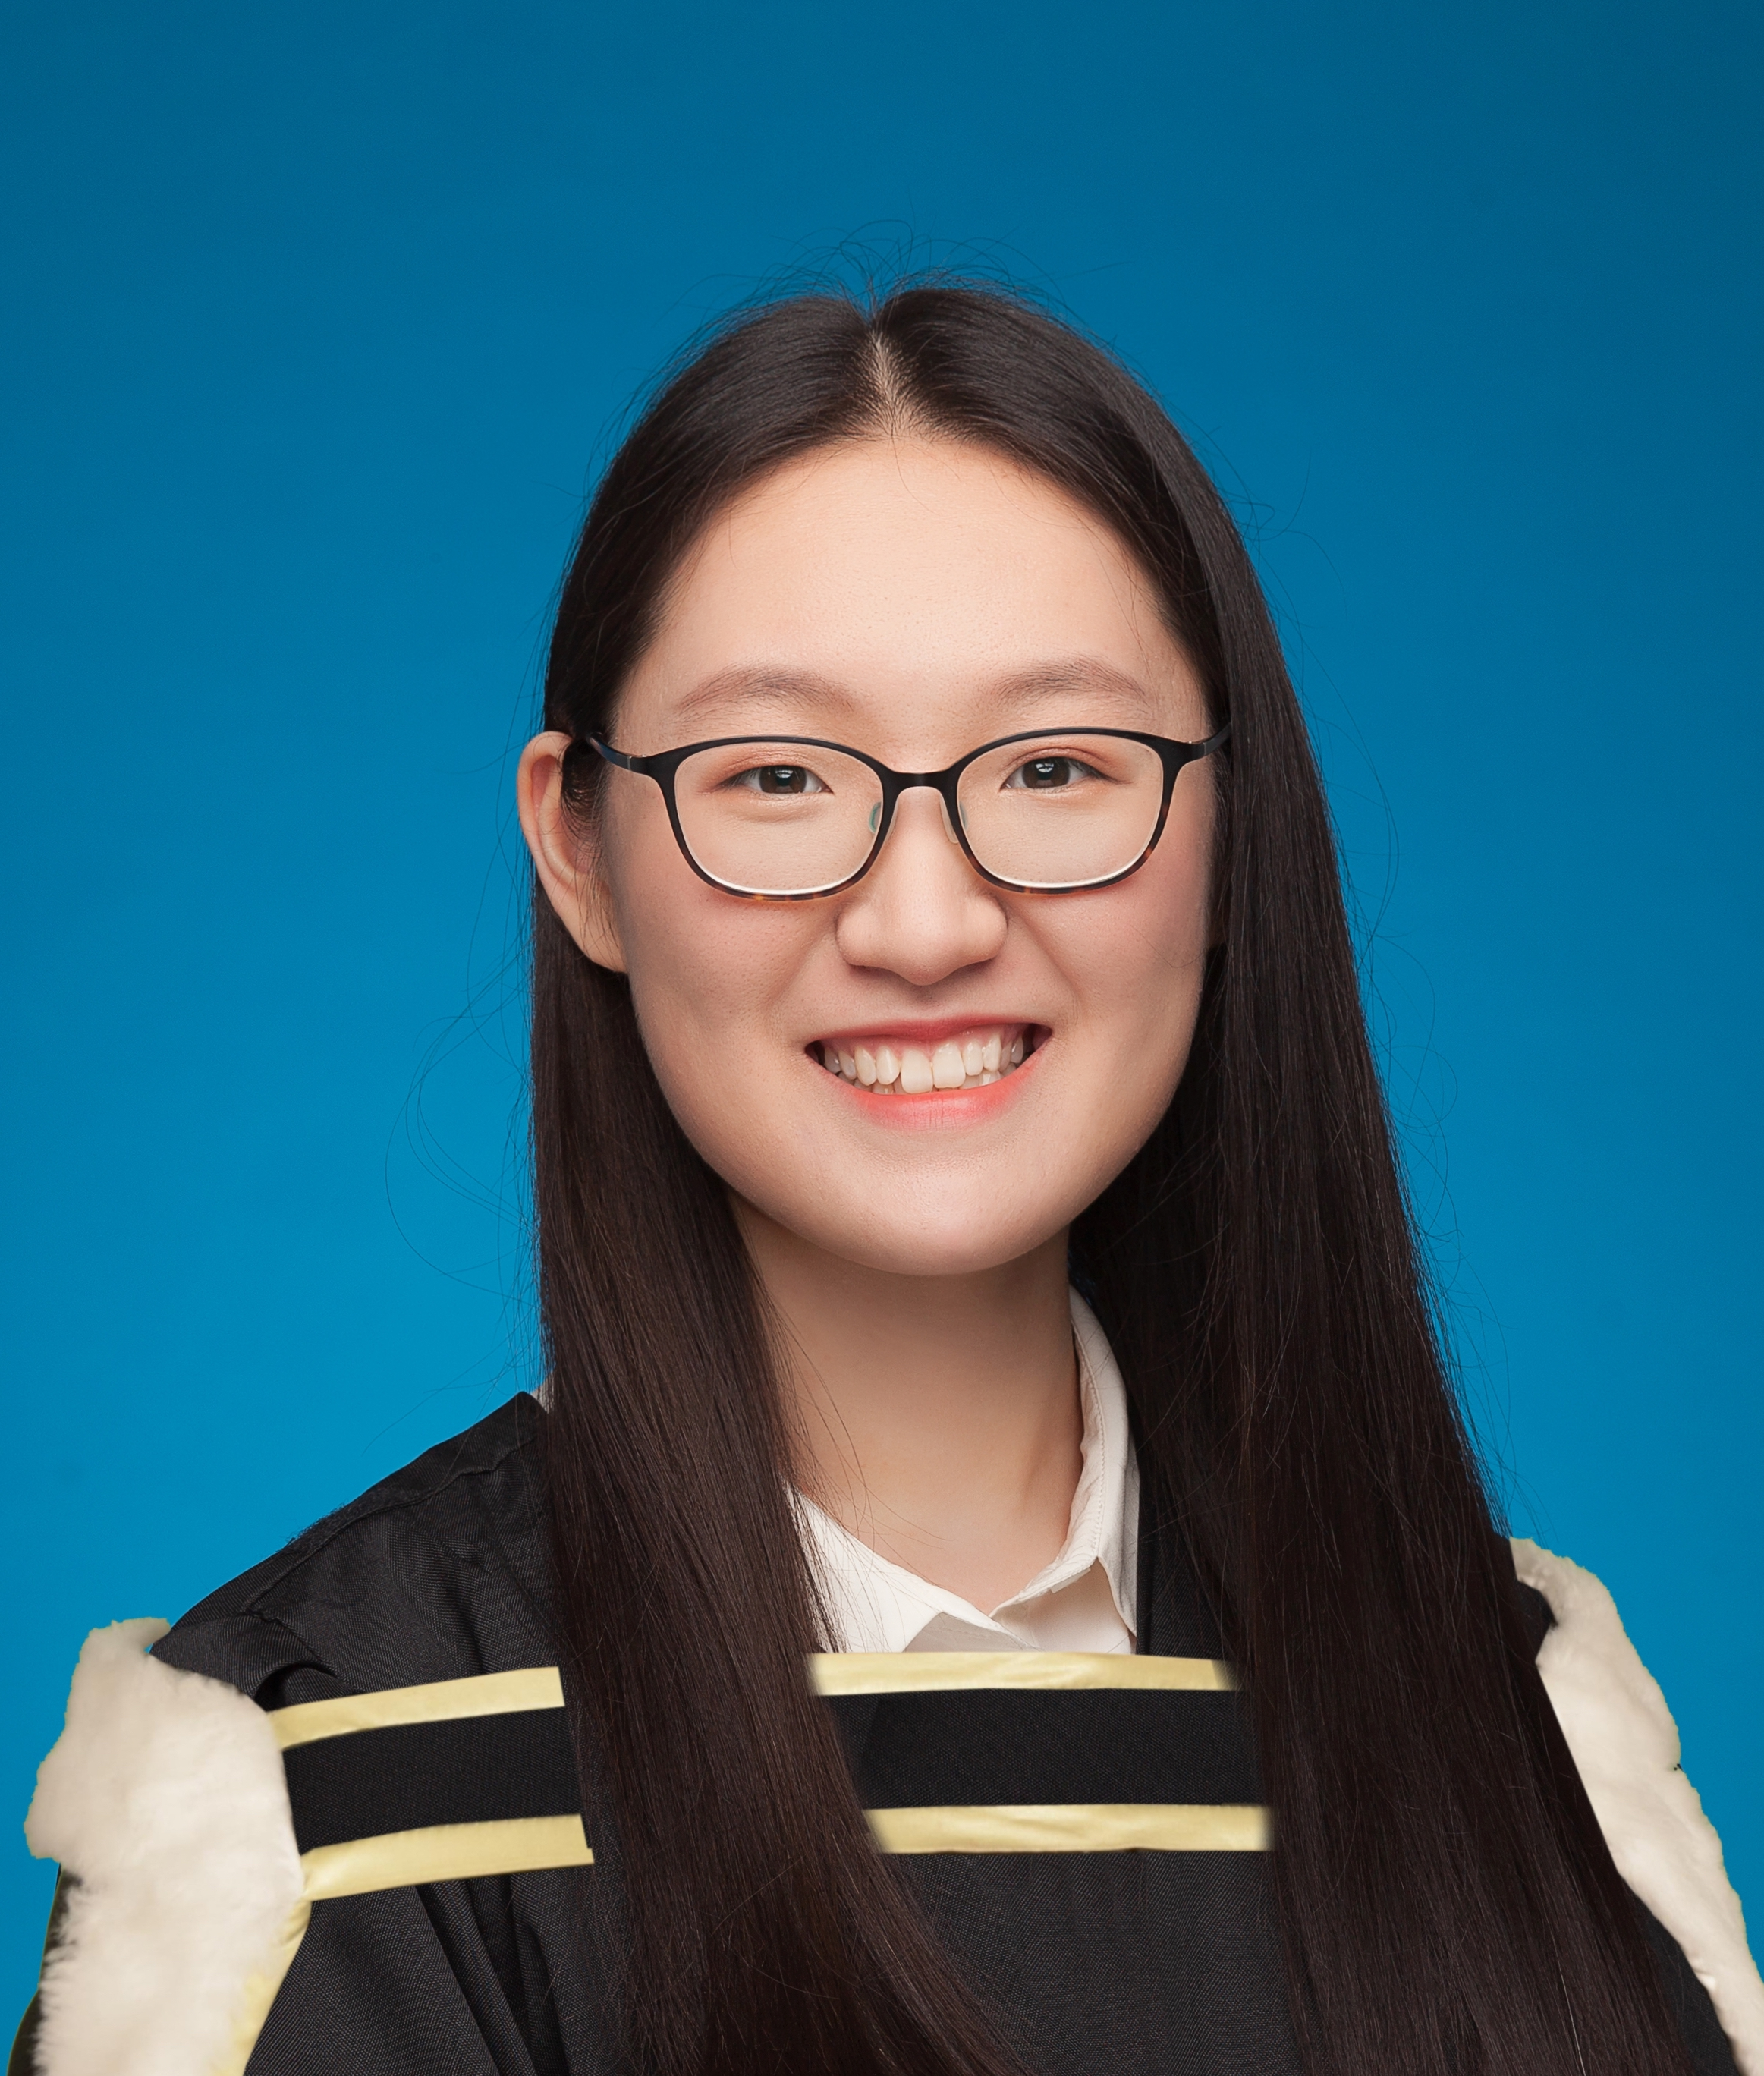
\includegraphics[width=0.20\textwidth]{images/me.jpg}
    \vspace{-2cm}\hspace{9cm} %move upward by 2cm, rightward by 2cm (same as moving right by 2,3,...10 cm, do not know why)
\end{wrapfigure} %width of the photo is 0.15 of the total width of page

\hfill\break


%\hfill\vspace{1cm}
\longcontact{\href{https://shimin233.github.io}{Github page 个人网页: https://shimin233.github.io} }{}{}{}{}
\vspace{-1.5cm}
\longcontact{}{}{地址:  上海市松江区洞泾镇洞塔路500弄49号201室}{邮箱: \href{mailto: sf686@cantab.ac.uk}{sf686@cantab.ac.uk}(剑桥大学 校友邮箱)}{手机:  +86 1881 759 5597}
%\vspace{-0.5cm}
\longcontact{}{}{Address:  Flat 3, Carthusian Court, 12 Carthusian St., London, EC1M 6EB, UK}{Email: \href{mailto: sf686@cantab.ac.uk}{sf686@cantab.ac.uk}}{Mobile:  +44 7579 946244}




\vspace{0.5cm}
\section{教育背景  EDUCATION}
\datedsubsection{硕士,纯数学 Master of Advanced Study, Pure Mathematics}{2020.10-2021.6}
\begin{itemize}
	\item 英国,剑桥郡,剑桥,剑桥大学,菲茨威廉姆学院,纯数学与数学统计系\\
		Dept. of Pure Mathematics and Mathematical Statistics, Fitzwilliam College, University of Cambridge, Cambridge, United Kingdom
	\item 总绩点66/满分100, 其中随机微积分与应用分数75/满分100。论文:随机推断的一个世纪 \\
	Overall mark 66/100. 75/100 in Stochastic Calculus \& Applications. Essay: A Century of Randomisation Inference
\end{itemize}

\lsubsection{理学士,荣誉数学,辅修经济 Bachelor of Science, Honours Mathematics, Minor Economics}{2016.9-2020.5}
\begin{itemize}
	\item 加拿大,魁北克省,蒙特利尔,麦吉尔大学,数学与统计系\\
	         Dept. of Mathematics and Statistics, McGill University, Montréal, QC, Canada
	\item 成绩与荣誉:数学一等荣誉,杰出毕业奖,Gowrisankaran数学/统计奖,绩点3.96/满分4.00\\
                  Grade and Prizes: First Class Honours in Mathematics, Grad Excellence Award, Gowrisankaran Prize in Math/Stats, GPA 3.96/4.00
\end{itemize}


\section{学术研究 RESEARCH PROJECTS \& ACADEMIC ACTIVITIES}

\datedsubsection{均匀生成树 \quad Uniform spanning tree}{2019.5-2019.8}
\begin{itemize}
    \item 指导教师: Louigi Addario-Berry;所属学校:加拿大,魁北克省,蒙特利尔,麦吉尔大学\\
    Supervisor: Louigi Addario-Berry, McGill University, Montréal, QC, Canada
    \item  研究内容:从配置模型、Pitman过程、马尔可夫链与混合时间、利用Lovász局部引理以均匀采样等多个角度,研究了均匀生成树与在图论领域的Aldous-Broder算法。\\
    Studies of uniform spanning trees and the Aldous-Broder algorithm on graphs, involving perspectives from configuration model, Pitman’s process, Markov chain and mixing, and uniform sampling through the Lovász Local Lemma.
\end{itemize}


\datedsubsection{树形检索及其应用 \quad Tree search and applications}{2019.1-2019.3}
\begin{itemize}
    \item 指导教师: Dmitry Jakobson;所属学校:加拿大,魁北克省,蒙特利尔,麦吉尔大学\\
    Supervisor: Dmitry Jakobson, McGill University, Montréal, QC, Canada
    \item 研究内容:研究广度优先搜索、深度优先搜索,并应用于寻找割点、图的区块方面;使用Kruskal算法与Prim算法以寻找最小生成树。\\
    Studies of  BFS, DFS, and their application in finding cut vertices and blocks of a graph; Kruskal’s algorithm and Prim’s algorithm in finding minimum-weight spanning trees. 
\end{itemize}

\datedsubsection{麦吉尔辅导阅读项目 \quad McGill Directed Reading Program (DRP)}{2019.1-2019.3}
\begin{itemize}
    \item 辅导者:Corentin Perret-Gentil;所属学校:加拿大,魁北克省,蒙特利尔,麦吉尔大学\\
    Mentor: Corentin Perret-Gentil, McGill University, Montréal, QC, Canada
    \item 通过与Corentin每周一对一的会面研究 “Futurama定理”。\\
    Studies of the "Futurama Theorem" in the weekly 1-on-1 meetings with Corentin.
\end{itemize}

\datedsubsection{蒙特利尔数学研究所探索学校:随机过程的动力学\quad Institut des Sciences Mathématiques (ISM) Discovery School-Dynamics of Random Processes}{2019.6}
\begin{itemize}
    \item 举办学校:加拿大,魁北克省,蒙特利尔,魁北克大学蒙特利尔校区\\
    L'Université du Québec à Montréal (UQAM), Montréal, QC, Canada
    \item  由来自牛津大学、麦吉尔大学、苏黎世联邦理工大学与柏林工业大学的多位教授一系列短课程与研讨会。\\
    A series of mini-courses and seminars was provided by multiple professors from Oxford, McGill, ETH Zürich and TU Berlin respectively.
\end{itemize}


\section{课外活动 EXTRA-CURRICULAR ACTIVITIES}

\datedsubsection{辅导员—麦吉尔数学帮助中心 \quad Helpdesk tutor}{2019.1-2019.5; 2019.9-2020.4}                       
\begin{itemize} 
	\item 加拿大,魁北克省,蒙特利尔,麦吉尔大学,数学与统计系,数学帮助中心\\
	The Math Helpdesk, Dept. of Math and Stats, McGill University, Montr\'eal, QC, Canada
	\item 每周辅导随时来求助的、多个专业的学生探究多个数学科目的问题\\
	Tutor the students who drop in, with a large variety of majors, in a wide range of math courses, every week.
 \end{itemize}

\datedsubsection{辅导员—学长辅导项目 \quad Mentor-Peer Mentor Buddy Program}{2019.9-2020.4}
\begin{itemize}
	 \item 加拿大,魁北克省,蒙特利尔,麦吉尔大学,数学与统计系\\
	 	Dept. of Math and Stats, McGill University, Montr\'eal, QC, Canada
	\item 作为高年级学生辅导员,对低年级学生一对一的帮助,提供合适的学习生活资源\\
		Provide peer support on a student-to-student level and refer mentees to appropriate resources 
\end{itemize}
 %=====To be re-formatted are following===========
\lsubsection{志愿者—麦吉尔国际学生帮助项目 \quad Volunteer-McGill International Student Buddy Program} {2018.9-2018.12; 2019.9-2020.4}
\begin{itemize} 
	\item 举办机构:加拿大,魁北克省,蒙特利尔,麦吉尔大学,国际学生服务\\
	International Student Services, McGill University, Montr\'eal, QC, Canada
	\item 作为注册志愿者在此项目中与新入学的国际学生配对,以在校生的角度提供关于麦吉尔大学与蒙特利尔的资源咨询\\
	The program pairs newly admitted international students with registered volunteers, who are resource people providing a current student perspective about life at McGill and in Montr\'eal.  
	\end{itemize}


\section{荣誉奖项 AWARDS \& SCHOLARSHIPS}
\datedsubsection{Gowrisankaran数学/统计奖 \quad Gowrisankaran Prize in Math/Stats}{2020.5}                                 
\begin{itemize} 
	\item  加拿大,魁北克省,蒙特利尔,麦吉尔大学,理科\\
	Faculty of Science, McGill University, Montr\'eal, QC, Canada
	\item 在2010年由Kohur Gowrisankaran教授及其亲友赞助为二年级或最高年级的、就读于全日制理科荣誉本科学位、攻读科目含有数学的杰出学生创立。 \\
	Established in 2010 by Professor Kohur Gowrisankaran with additional contributions from family and friends for outstanding students in their second or final year of a full-time Honours undergraduate degree program in the Faculty of Science with Mathematics as at least one component.
\end{itemize} 



\datedsubsection{理科院长荣誉名单\quad Dean’s Honour List}{2017.8; 2019.8}                                 
\begin{itemize} 
	\item 加拿大,魁北克省,蒙特利尔,麦吉尔大学,理科\\
	Faculty of Science, McGill University, Montr\'eal, QC, Canada
	\item 大学对于学生成就的官方认证,此认证会被记录在成绩单上。颁发给不超过前10\%的学生。\\
	An official University recognition of the student's achievements and is recorded on the transcript. Conferred upon no more than the top 10\% of students.
\end{itemize} 

\datedsubsection{Jeanne Bell理科本科生研究奖,与数学统计本科生奖 \quad Jeanne Bell Science Undergraduate Research Award, and Math \& Stat Undergrad Award as Science Undergraduate Research Awards (SURAs)}{2019.5-2019.8 }  
\begin{itemize} 
	\item 加拿大,魁北克省,蒙特利尔,麦吉尔大学,理科\\
	Faculty of Science, McGill University, Montr\'eal, QC, Canada 
	\item 获奖者在麦吉尔的一位理科教授指导与资金支持下,参与16周的全日制研究,获得学术研究的相关经验。\\
	Recipients engage in a 16-week full-time research and development activity to gain experience in academic research, under supervision of a McGill science professor and with financial support. 
\end{itemize} 

 

\datedsubsection{Brennen, Herbert奖学金 \quad Brennen, Herbert Scholarships}{2019.8}                                                  
\begin{itemize} 
	\item 加拿大,魁北克省,蒙特利尔,麦吉尔大学,理科\\
	Faculty of Science, McGill University, Montr\'eal, QC, Canada
	\item 在1992年由1919年校友,理学士H.J. Brennen遗赠,为主修化学或数学的杰出学生建立。由理科奖学金委员会颁发。\\
	Established in 1992 by a bequest from H.J. Brennen, B.Sc. 1919, for deserving students majoring in Chemistry or Mathematics. Awarded by the Faculty of Science Scholarships Committee.\end{itemize}

 
\datedsubsection{Tomlinson本科生奖 \quad Tomlinson Undergraduate Award}{2019.4, 2019.7, 2019.12; 2020.4}                                                   
\begin{itemize} 
	\item 加拿大,魁北克省,蒙特利尔,麦吉尔大学,理科\\
	Faculty of Science, McGill University, Montr\'eal, QC, Canada
	\item 为了加强本科生的教育质量,担任学生辅导员,贡献教学资源。\\
	In order to enhance the quality of education received by undergraduate students, improve the teaching resources for courses as one of the peer-mentors. 
\end{itemize}

\datedsubsection{理科奖学金 \quad Faculty of Science Scholarships}{2017.8}
\begin{itemize} 
	\item 加拿大,魁北克省,蒙特利尔,麦吉尔大学,理科\\
	Faculty of Science, McGill University, Montr\'eal, QC, Canada
	\item 在1992年由大学建立以表彰科系中前5\%的学生的学术成就。\\
	Established in 1992 by the University to provide awards based on academic achievement to students in the top 5\% of the Faculty. 
\end{itemize}

\section{技能特长 SKILLS \& INTERESTS}
\vspace{-0.5em}
\textbf{软件技能 Skills}
\begin{itemize}[topsep=-1em, itemsep=0.3em, parsep=0pt, partopsep=1em]
	  \item \LaTeX, Python, Markdown, R (基础basic) , MySQL (基础basic), 正在进一步学习编程并使用Github做笔记 actively leaning programming with notes on Github; MS Word, Excel, Powerpoint and Outlook;
	\item 使用Adobe Flash and Photoshop制作动画与图像; HTML \& CSS, 有网页与logo设计的经验\\
	Adobe Flash and Photoshop experience, designing webpages, logos. % Microsoft Word, Excel, Powerpoint and Outlook?
\end{itemize}

\vspace{1em}
\textbf{语言技能 Languages}
\begin{itemize}[topsep=-1em, itemsep=0.3em, parsep=0pt, partopsep=1em]
	\item  中文(母语);英语(流利);法语(基础)\\
	Chinese (Mandarin) (native); English (fluent); French (basic).
\end{itemize}

\vspace{1em}
\textbf{兴趣特长 Interests}
\begin{itemize}[topsep=0em, itemsep=0.3em, parsep=0pt, partopsep=1em]
	\item 热衷于数学研究与现实中人类活动的互动,以及向大众介绍数学的艺术。\\
	Enthusiasm in interaction between Maths researches and real-world human activities, and introducing the art of Maths to public. 
	\item 二胡【17年】;中文硬笔书法与西方拉丁字母书法;摄影;滑冰;爵士舞。\\
	Erhu (Chinese traditional musical instrument)[15 years]; Chinese and Western calligraphy; photography; ice-skating; Jazz dance. 
\end{itemize}

\end{document}  

%=====Comments given by this XeLaTeX template=====

% XeLaTeX can use any Mac OS X font. See the setromanfont command below.
% Input to XeLaTeX is full Unicode, so Unicode characters can be typed directly into the source.

% The next lines tell TeXShop to typeset with xelatex, and to open and save the source with Unicode encoding.

%!TEX TS-program = xelatex
%!TEX encoding = UTF-8 Unicode

%====

% For many users, the previous commands will be enough.
% If you want to directly input Unicode, add an Input Menu or Keyboard to the menu bar 
% using the International Panel in System Preferences.
% Unicode must be typeset using a font containing the appropriate characters.
% Remove the comment signs below for examples.

% \newfontfamily{\A}{Geeza Pro}
% \newfontfamily{\H}[Scale=0.9]{Lucida Grande}
% \newfontfamily{\J}[Scale=0.85]{Osaka}

% Here are some multilingual Unicode fonts: this is Arabic text: {\A السلام عليكم}, this is Hebrew: {\H שלום}, 
% and here's some Japanese: {\J 今日は}.
